\section{Spécifications}

\subsection{Caractérisation de l'environnement}

Il s'agit dans cette partie de caractériser l'environnement c'est-à-dire de d'identifier les entités interagissant avec le circuit à concevoir et décrire leur évolution à l'aide d'automates.
L'environnement du circuit à concevoir est constitué de trois entités :

\begin{itemize}
	\item Le processeur
	\item Le contrôleur mémoire fournissant le signal de sélection nCS\_IT.
	\item Les 15 entités informant au contrôleur d'interruptions la présence d'une interruption.
	      Ce groupe d'entités est appelé "source d'interruptions".
\end{itemize}

L'ensemble processeur + contrôleur mémoire peut configurer le contrôleur d'interruptions et opérer des écritures et lectures au sein de ses registres.
Cet ensemble sera par la suite nommé "système à microprocesseur".
L'entité source d'interruptions envoie au circuit à concevoir la présence d'une interruption à traiter.

\begin{figure}[H]
	\centering
	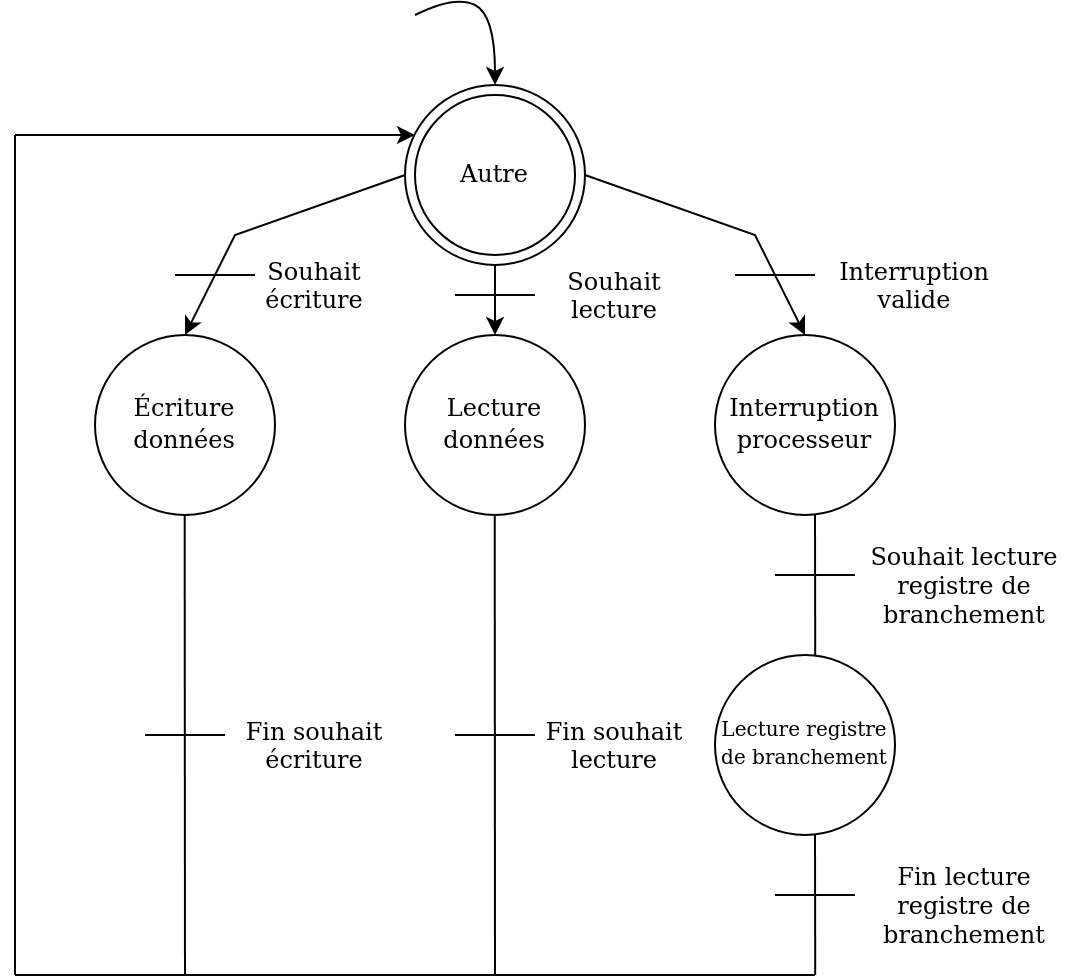
\includegraphics[width=0.8\linewidth]{figure/spec_automate_proc_ctrlmem.png}
	\caption{Comportement du système à microprocesseur}
	\label{fig:spec_automate_sysmicro}
\end{figure}

La figure ci-dessus représente le comportement de l'entité système à microprocesseur.
Celui-ci possède trois cycles de fonctionnement.
Le processeur peut opérer des cycles de lecture et d'écriture dans les registres du contrôleur d'interruptions.
Le souhait d'écriture ou de lecture s'effectue par la mise à l'état bas du signal nCS\_IT.
La fin de ces cycles est notifiée par la mise à l'état haut du signal nAS.
Le terme "données" peut signifier la valeur des registres de configuration et également l'adresse de branchements.\\


\begin{figure}[H]
	\centering
	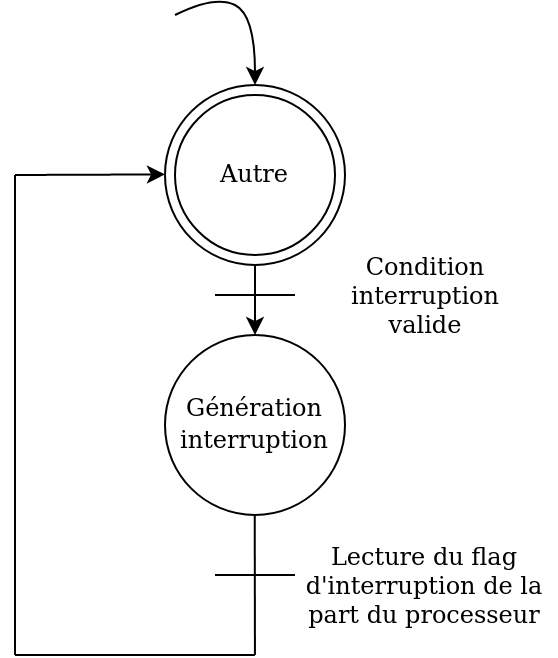
\includegraphics[width=0.5\linewidth]{figure/spec_automate_src_int.png}
	\caption{Comportement de l'entité source d'interruptions}
	\label{fig:spec_automate_src_it}
\end{figure}

La figure ci-dessus est l'automate de l'entité source d'interruptions.
Lorsque la condition d'interruption est valide, le périphérique génère un signal en direction du contrôleur d'interruptions.
Ce signal reste actif jusqu'à la lecture du flag d'interruption de la part du processeur.

\subsection{Entrées et sorties du composant}

La caractérisation de l'environnement sous forme d'automates donne les relations d'entrées et sorties du circuit à concevoir avec les diverses entités.
Il est alors possible de présenter de manière structurelle le circuit à concevoir et les entités de l'environnement.

\begin{figure}[H]
	\centering
	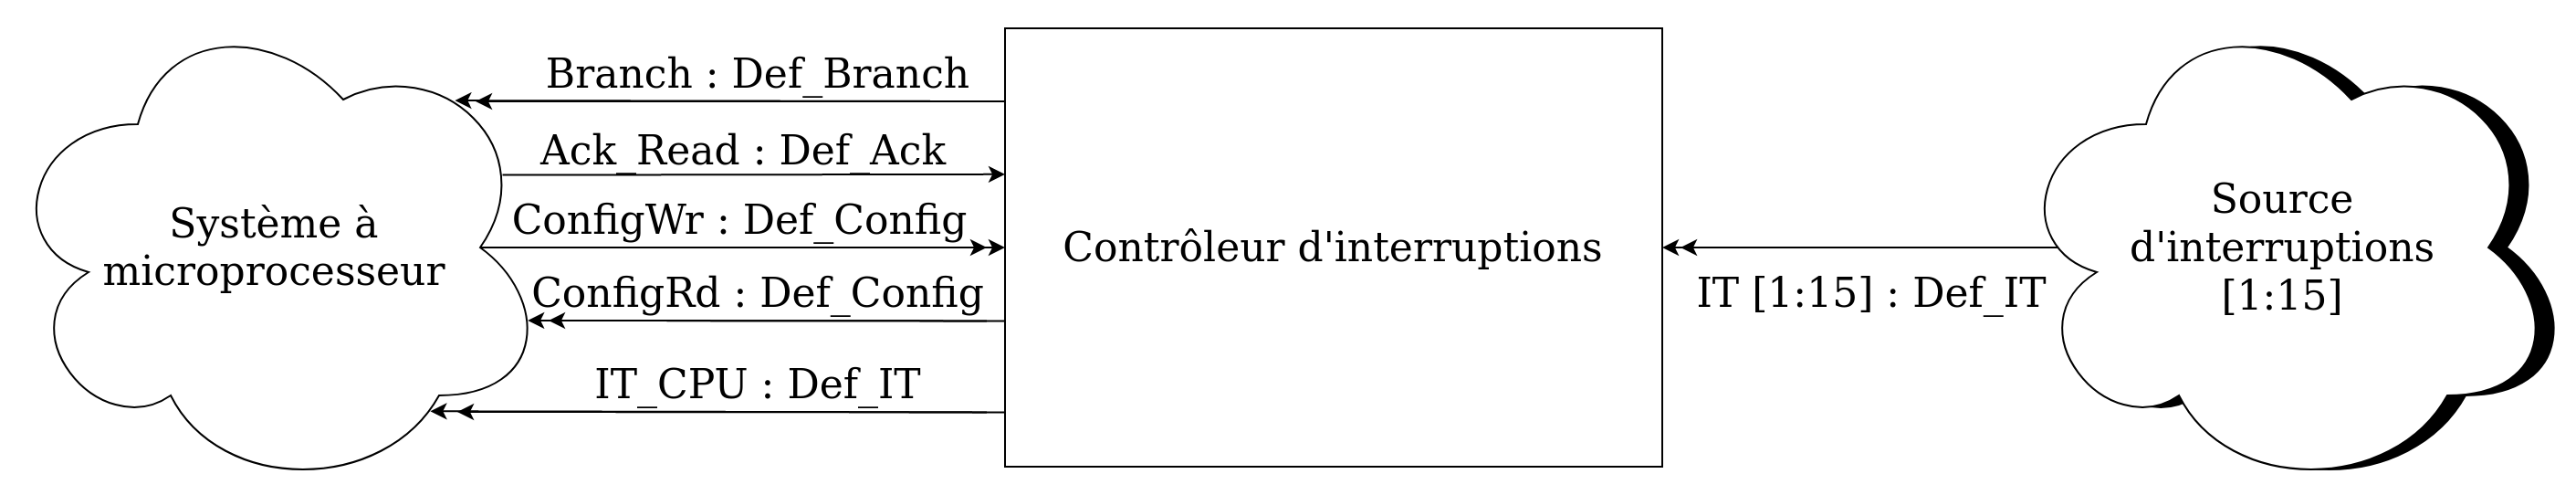
\includegraphics[width=1\linewidth]{figure/entrees_sorties_composant.png}
	\caption{Entrées et sorties du circuit à concevoir}
	\label{fig:entrees_sorties_composant}
\end{figure}

Le tableau ci-dessous récapitule les relations avec leur sens, leur catégorie et leur type.

\begin{table}[H]
	\centering
	\begin{tabular}{|c|c|c|c|c|}
		\hline
		Entités                       & Relation  & Catégorie    & Sens   & Type          \\
		\hline
		                              & Branch    & Permanent    & Sortie & Def\_Branch   \\
		                              & Ack\_Read & Évènementiel & Entrée & Def\_Ack      \\
		Système à microprocesseur     & ConfigWr  & Permanent    & Entrée & Def\_ConfigWr \\
		                              & ConfigRd  & Permanent    & Sortie & Def\_ConfigRd \\
		                              & IT\_CPU   & Permanent    & Sortie & Def\_IT       \\
		\hline
		Source d'interruptions [1:15] & IT [1:15] & Permanent    & Entrée & Def\_IT       \\
		\hline
	\end{tabular}
	\caption{Sens et rôle des signaux}
	\label{tab:entrees_sorties_composant}
\end{table}

La relation Ack\_Read est de type Def\_Ack, une donnée de type booléen (true : la lecture de l'adresse de branchement est terminée, false sinon).
IT[1:15] est un tableau de 15 éléments de type Def\_IT, une donnée de type booléen (true : une interruption est reçu de la part de n-ième l'IP, false sinon).
IT\_CPU est également de type Def\_IT (true : une interruption doit être traitée par le CPU, false sinon).
Chaque autre relation est une composition de sous-relations comme définie ci-après.

\begin{equation*}
\mbox{Branch} = \mbox{ ID } + \mbox{ @blx }
\end{equation*}

\begin{equation*}
\mbox{ConfigWr} = \mbox{ @handler } + \mbox{ priorité } + \mbox{ masque }
\end{equation*}

\begin{equation*}
\mbox{ConfigRd} = \mbox{ ID } + \mbox{ @handler } + \mbox{ @blx } + \mbox{ priorité } + \mbox{ masque } + \mbox{ pending } + \mbox{ traitement }
\end{equation*}

ID représente l'identifiant de l'interruption.
@blx est la sous-relation qui précise l'adresse de branchement de la sous-routine de l'interruption à traiter. @handler est un tableau comportant les adresses des sous-routines d'interruptions.
La relation priorité indique la priorité attribuée pour une interruption, masque précise si l'interruption est masquée ou non.
En ce qui concerne pending, il s'agit d'une sous-relation qui informe si une interruption est mise en attente pour être traitée ultérieurement.
Enfin, traitement prends en compte si une interruption a déjà été traitée ou non avant que celle-ci soit clear par l'IP concernée.

\begin{table}[H]
	\centering
	\begin{tabular}{|c|c|c|}
		\hline
		Sous-relation & Type            & Donnée                              \\
		\hline
		& & \\
		ID & Def\_ID & Entier de 0 à 14\\
		& & \\
		\hline
		& & \\
		@blx & Def\_@blx & Entier de 0 à $2^{22}-1$\\
		& & \\
		\hline
		& & Tableau de 30 éléments de taille\\
		@handler & Def\_@handler & Def\_Data valant 16$\times$Def\_Bit\\
		& & avec Def\_Bit 0 ou 1\\
		\hline
		& & Entier de 0 à 7\\
		priorité & Def\_priorité & 0 : le plus prioritaire\\
		& & 7 : le moins prioritaire\\
		\hline
		              &                 & Booléen                             \\
		masque        & Def\_masque     & true : IT masquée (prise en compte) \\
		              &                 & false : non masquée                 \\
		\hline
		              &                 & Booléen                             \\
		pending       & Def\_pending    & true : IT mise en attente           \\
		              &                 & false sinon                         \\
		\hline
		              &                 & Booléen                             \\
		traitement    & Def\_traitement & true : IT à traiter                 \\
		              &                 & false : IT déjà traitée             \\
		\hline
	\end{tabular}
	\caption{Sous-relations et type de données}
	\label{tab:sous-relation}
\end{table}

Il est possible d'introduire une relation interne nommée infoIT. Le k-ième élément de infoIT correspond à la k-ième interruption, c'est-à-dire la valeur de ID. Cet indice k varie de 0 à 14 (0-14 représentant les 15 interruptions).

\begin{equation*}
	\mbox{infoIT[k]} = \mbox{ ID } + \mbox{ priorité } + \mbox{ masque } + \mbox{ pending } + \mbox{ traitement }
\end{equation*}

\newpage

\subsection{Spécifications fonctionnelles}
Les spécifications fonctionnelles comprennent la liste des fonctions du système
pour l'application (fonctions externes) et la description du comportement du système et
de l'environnement pour ces fonctions \cite{Calvez_2}.

\gap

La fonction première du contrôleur d'interruption est d'informer le processeur lorsqu'une interruption valide survient.
Une interruption valide est définie comme étant non masquée et de niveau suffisant pour être prise en compte.
La gestion des niveaux de priorité est la seconde fonction à considérer.
Elle est directement induite par la première.
Une interruption en cours ne peut être interrompue que par une interruption de niveau strictement supérieur.
Lorsque le processeur acquitte la fin du traitement, les interruptions de niveaux inférieurs ou égaux peuvent être à nouveau considérées comme valides.
Le contrôleur fournir un niveau de priorité par défaut pour chaque source.
La troisième fonction concerne le masquage des sources d'interruption individuellement.
Une source masquée ne génèrera pas de signal au processeur.
Un événement déjà en cours de traitement par le contrôleur ne pourra être masqué. %TODO à confirmer
Si un signal d'interruption est généré alors qu'il est masqué, il est ignoré, mais s'il est démasqué alors qu'il est toujours actif alors il sera pris en compte. (\hl{A confirmer})
La quatrième fonction principale spécifie le vecteur d'exception.
Le contrôleur lorsque qu'il informe le processeur doit immédiatement lui indiquer vers quelle adresse il doit brancher.
Il est possible de configurer une adresse par source.
Sa configuration doit se faire lorsque le contrôleur est désactivé.
Si aucune adresse n'est présente pour une source donnée alors une par défaut sera attribuée.

\begin{table}[H]
	\centering
	\begin{tabular}{|c|c|}
		\hline
		nom & Description                          \\ \hline
		fn1 & Informer le processeur               \\ \hline
		fn2 & Gérer les niveaux de priorité        \\ \hline
		fn3 & Masquer individuellement les sources \\ \hline
		fn4 & Configurer le vecteur d'exception    \\ \hline
	\end{tabular}
	\caption{Synthèse des spécifications fonctionnelles}
	\label{tab:spe_funct}
\end{table}

Le tableau \ref{tab:spe_funct} synthétise les spécifications fonctionnelles.
Il permet de contrôler que chaque point est bien traité tout au long de la conception.
Il n'est cependant pas précis et devra être traité avec la description détaillée ci-dessus.

\begin{figure}[H]
	\centering
	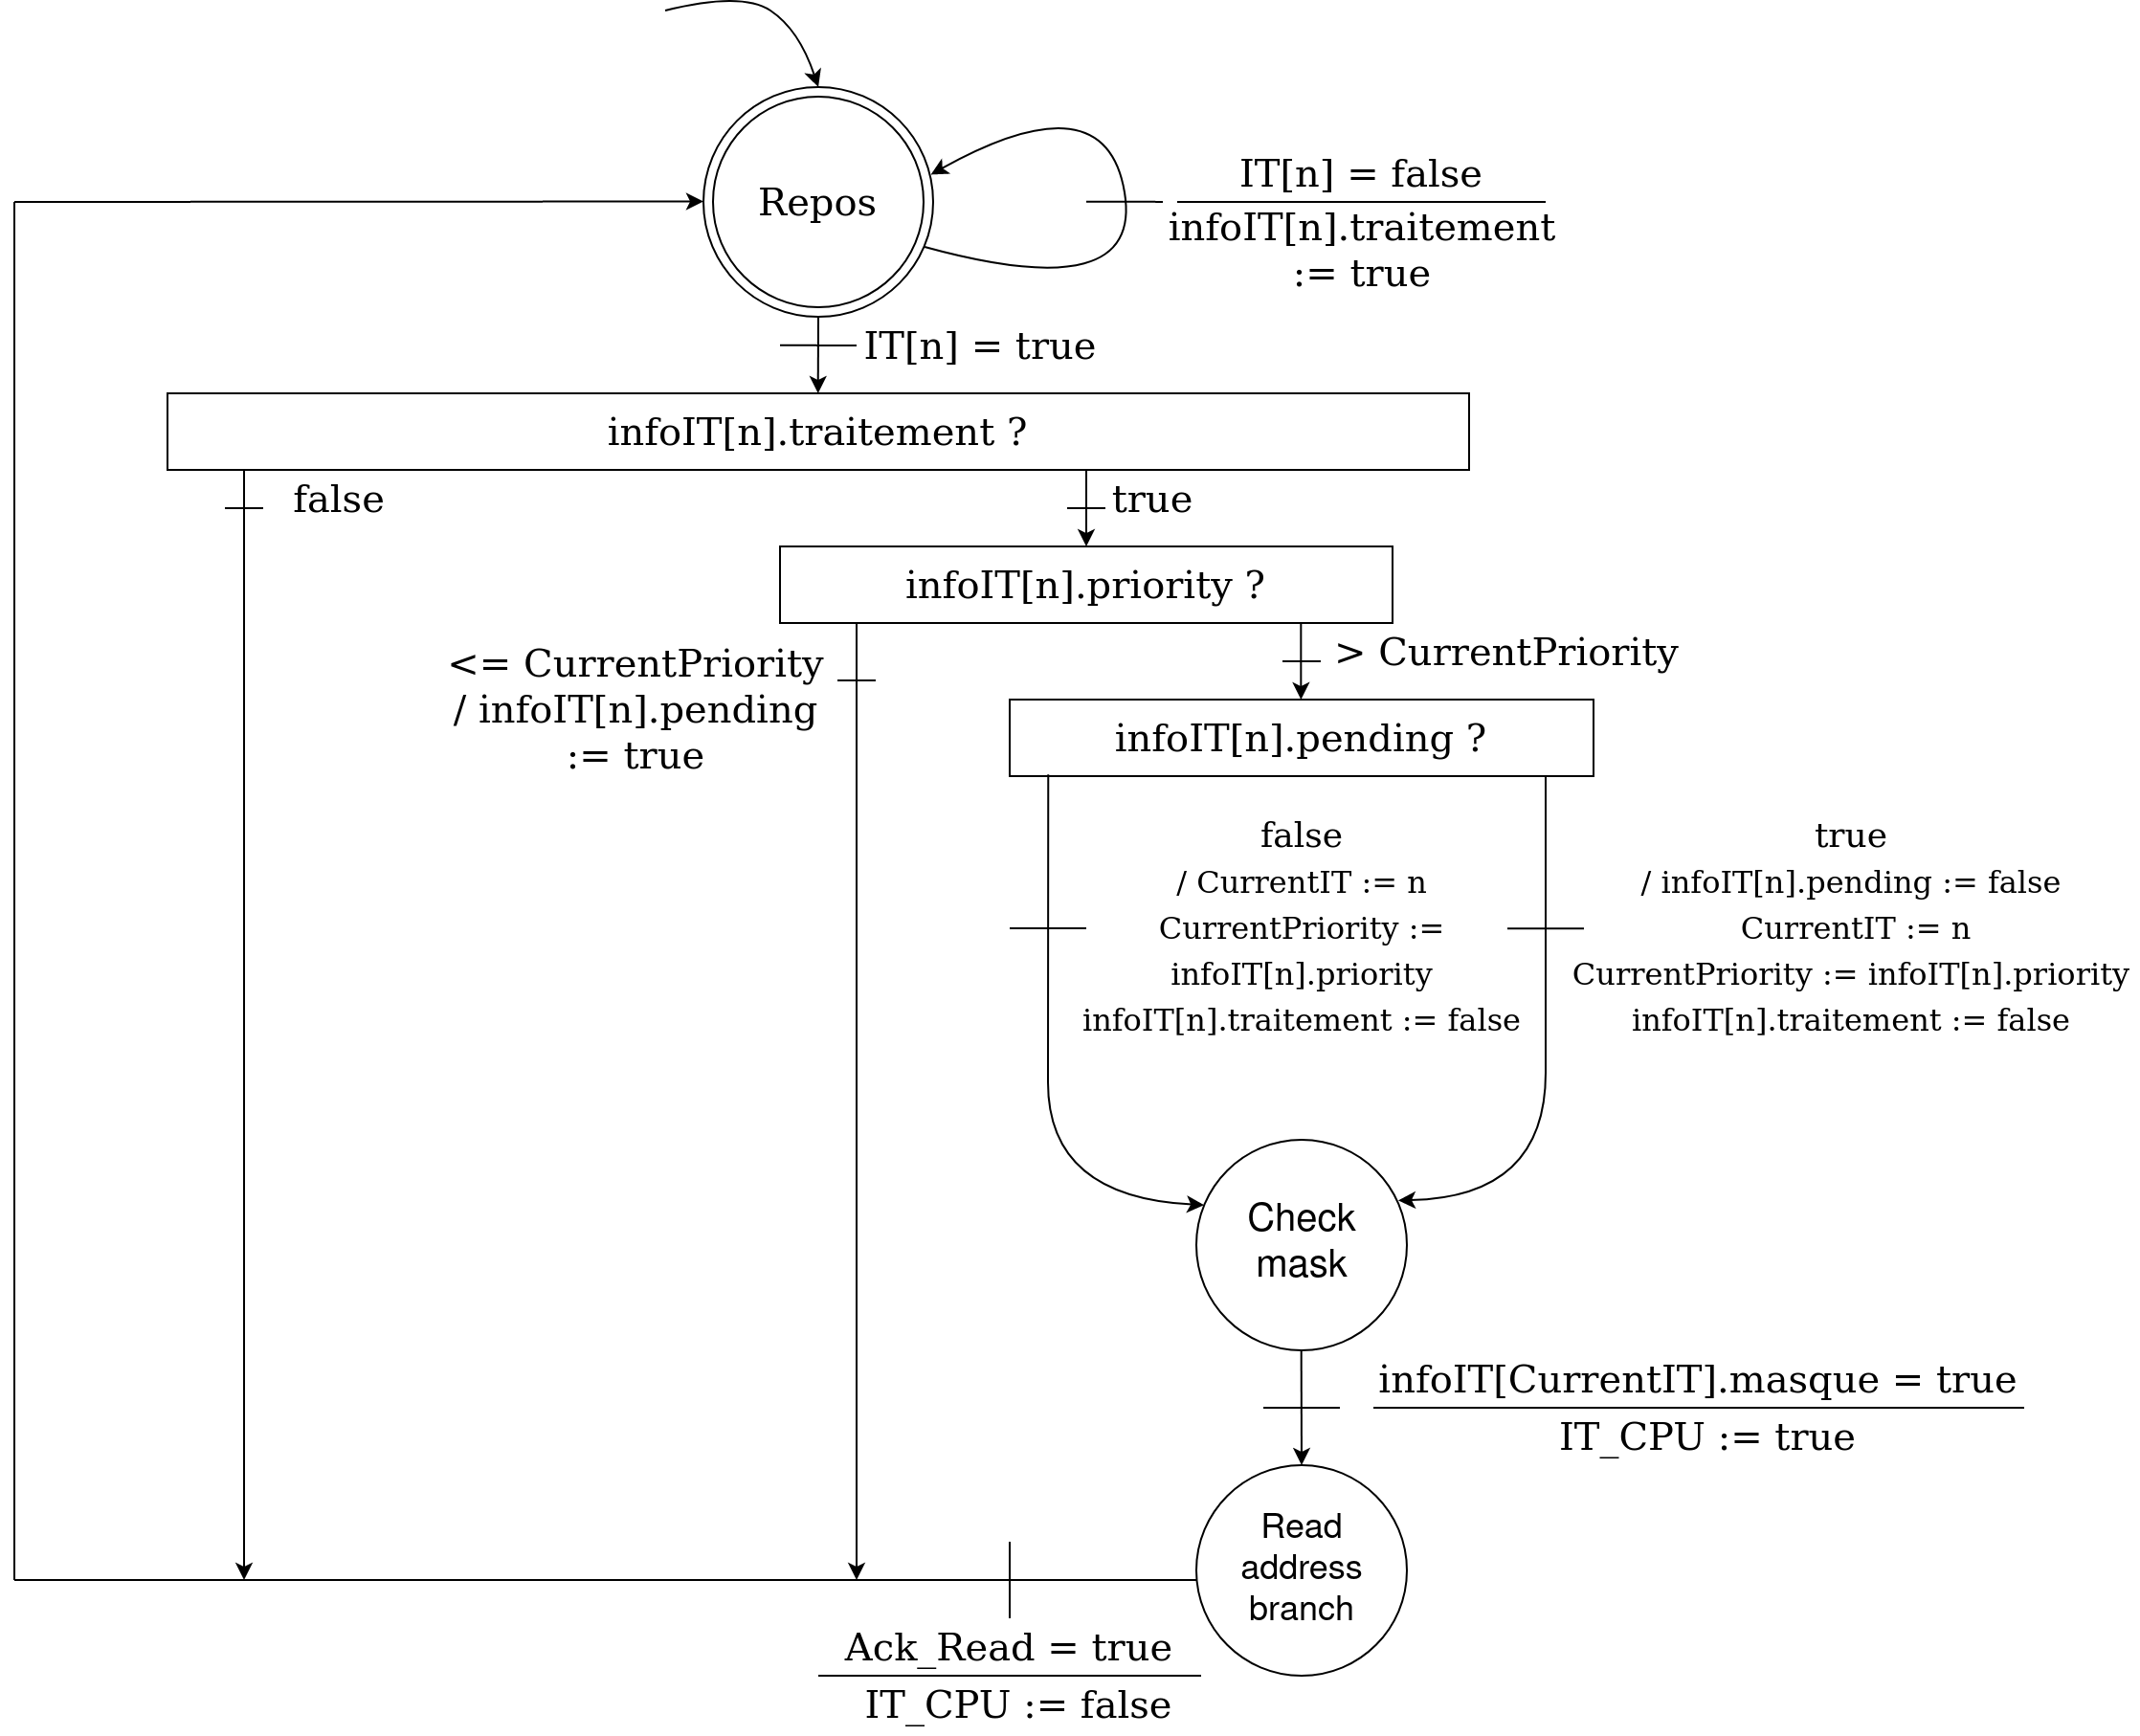
\includegraphics[width=1\linewidth]{figure/spec_fonc_1.png}
	\caption{Automate du contrôleur d'interruptions}
	\label{fig:spec_func_1}
\end{figure}

\begin{table}[H]
	\centering
	\begin{tabular}{|c|c|c|}
		\hline
		ID & Interruptions correspondantes & Adresses de branchement par défaut\\
		\hline
		0 & nIT\_ext0 & \\
		\hline
		1 & nIT\_ext1 & \\
		\hline
		2 & nIT\_ext2 & \\
		\hline
		3 & nIT\_ext3 &\\
		\hline
		4 & nIT\_RTC &\\
		\hline
		5 & nIT\_TC\_PWM &\\
		\hline
		6 & nIT\_pos\_vit &\\
		\hline
		7 & nIT\_FFTA &\\
		\hline
		8 & nIT\_NNA &\\
		\hline
		9 & nIT\_SPI &\\
		\hline
		10 & nIT\_PCI &\\
		\hline
		11 & nIT\_UART &\\
		\hline
		12 & nIT\_I2C &\\
		\hline
		13 & nIT\_CAN &\\
		\hline
		14 & nIT\_DMA &\\
		\hline
	\end{tabular}
	\caption{Vecteurs d'interruptions}
	\label{tab:vec_int}
\end{table}


%\begin{figure}[H]
%	\centering
%	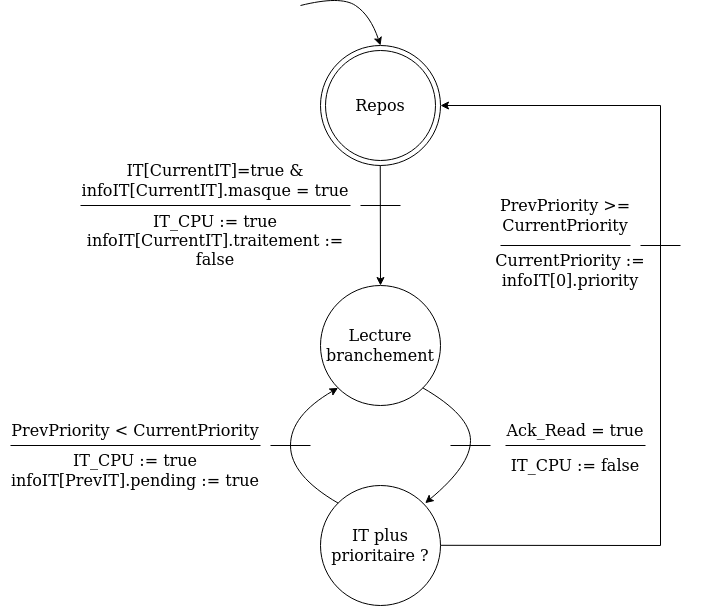
\includegraphics[width=0.9\linewidth]{figure/spec_fonc_2.png}
%	\caption{Second automate du contrôleur d'interruptions}
%	\label{fig:spec_func_2}
%\end{figure} 

\subsection{Spécification des registres}
Le tableau \ref{tab:reg_map} ci-dessous donne l'organisation des registres dans le contrôleur.
Une vue détaillée par chacun d'eux est présentée ensuite.
\newpage
\begin{table}[H]
	\centering
	\begin{tabular}{llllll}
		\hline
		\addlinespace[1ex] %Space between lines for tables
		\textbf{Adresse}     & \textbf{Nom}           & \textbf{Type} & \textbf{Reset} & \textbf{Description}                 \\
		\rhline
		\texttt{0x00000000}  & CTRL\_IT\_EN           & RW            & 0x0000         & Registre activation contrôlleur d'IT \\
		\rhline
		\texttt{0x00000002}  & CTRL\_IT\_MSQ          & RW            & 0x0000         & Registre de masquage                 \\
		\rhline
		\texttt{0x00000004}  & CTRL\_IT\_PEND         & R             & 0x0000         & Registre IT suspendues (pending)     \\
		\rhline
		\texttt{0x00000006-} & CTRL\_IT\_BRA          & R             & 0x0000         & Registre de branchement              \\
		\texttt{0x00000008}  &                        &               &                &                                      \\
		\rhline
		\texttt{0x0000000A-} & CTRL\_IT\_ADDR\_0      & RW            & 0x0000         & Adresses de branchement ch 0         \\
		{0x0000000C}         &                        &               &                &                                      \\
		\rhline
		\texttt{0x0000000E-} & CTRL\_IT\_ADDR\_1      & RW            & 0x0000         & Adresses de branchement ch 1         \\
		{0x00000010}         &                        &               &                &                                      \\
		\rhline
		\texttt{0x00000012-} & CTRL\_IT\_ADDR\_2      & RW            & 0x0000         & Adresses de branchement ch 2         \\
		{0x000000014}        &                        &               &                &                                      \\
		\rhline
		\texttt{0x00000016-} & CTRL\_IT\_ADDR\_3      & RW            & 0x0000         & Adresses de branchement ch 3         \\
		{0x000000018}        &                        &               &                &                                      \\
		\rhline
		\texttt{0x0000001A-} & CTRL\_IT\_ADDR\_4      & RW            & 0x0000         & Adresses de branchement ch 4         \\
		{0x0000001C}         &                        &               &                &                                      \\
		\rhline
		\texttt{0x0000001E-} & CTRL\_IT\_ADDR\_5      & RW            & 0x0000         & Adresses de branchement ch 5         \\
		{0x00000020}         &                        &               &                &                                      \\
		\rhline
		\texttt{0x00000022-} & CTRL\_IT\_ADDR\_6      & RW            & 0x0000         & Adresses de branchement ch 6         \\
		{0x000000024}        &                        &               &                &                                      \\
		\rhline
		\texttt{0x00000026-} & CTRL\_IT\_ADDR\_7      & RW            & 0x0000         & Adresses de branchement ch 7         \\
		{0x00000028}         &                        &               &                &                                      \\
		\rhline
		\texttt{0x0000002A-} & CTRL\_IT\_ADDR\_8      & RW            & 0x0000         & Adresses de branchement ch 8         \\
		{0x0000002C}         &                        &               &                &                                      \\
		\rhline
		\texttt{0x0000002E-} & CTRL\_IT\_ADDR\_9      & RW            & 0x0000         & Adresses de branchement ch 9         \\
		{0x00000030}         &                        &               &                &                                      \\
		\rhline
		\texttt{0x00000032-} & CTRL\_IT\_ADDR\_10     & RW            & 0x0000         & Adresses de branchement ch 10        \\
		{0x00000034}         &                        &               &                &                                      \\
		\rhline
		\texttt{0x00000036-} & CTRL\_IT\_ADDR\_11     & RW            & 0x0000         & Adresses de branchement ch 11        \\
		{0x00000038}         &                        &               &                &                                      \\
		\rhline
		\texttt{0x0000003A-} & CTRL\_IT\_ADDR\_12     & RW            & 0x0000         & Adresses de branchement ch 12        \\
		{0x0000003C}         &                        &               &                &                                      \\
		\rhline
		\texttt{0x0000003E-} & CTRL\_IT\_ADDR\_13     & RW            & 0x0000         & Adresses de branchement ch 13        \\
		{0x00000040}         &                        &               &                &                                      \\
		\rhline
		\texttt{0x00000042-} & CTRL\_IT\_ADDR\_14     & RW            & 0x0000         & Adresses de branchement ch 14        \\
		{0x00000044}         &                        &               &                &                                      \\
		\rhline
		\texttt{0x00000046}  & CTRL\_IT\_PRIO\_0\_1   & RW            & 0x0000         & Registre des priorités               \\
		\rhline
		\texttt{0x00000048}  & CTRL\_IT\_PRIO\_2\_3   & RW            & 0x0000         & Registre des priorités               \\
		\rhline
		\texttt{0x0000004A}  & CTRL\_IT\_PRIO\_4\_5   & RW            & 0x0000         & Registre des priorités               \\
		\rhline
		\texttt{0x0000004C}  & CTRL\_IT\_PRIO\_6\_7   & RW            & 0x0000         & Registre des priorités               \\
		\rhline
		\texttt{0x0000004E}  & CTRL\_IT\_PRIO\_8\_9   & RW            & 0x0000         & Registre des priorités               \\
		\rhline
		\texttt{0x00000050}  & CTRL\_IT\_PRIO\_10\_11 & RW            & 0x0000         & Registre des priorités               \\
		\rhline
		\texttt{0x00000052}  & CTRL\_IT\_PRIO\_12\_13 & RW            & 0x0000         & Registre des priorités               \\
		\rhline
		\texttt{0x00000054}  & CTRL\_IT\_PRIO\_14     & RW            & 0x0000         & Registre des priorités               \\
		\hline
	\end{tabular}
	\caption{Organisation des registres du contrôleur d'interruption (vue globale)}
	\label{tab:reg_map}
\end{table}

Le regitre CTRL\_IT\_EN contrôle l'activation de la partie opérative du composant. Lorsque le bit \texttt{Enable} vaut zero, les interruptions ne sont plus prises en compte, il est toujours possible d'écrire et lire l'état des registres.

\begin{table}[H]
	\centering
	\begin{tabular}{lll}
		\toprule
		\textbf{Bit} & \textbf{Nom} & \textbf{Fonction}                                 \\ \midrule
		$[0]$        & Enable       & Active ou lit l'état d'activation du périphérique \\
		             &              &
		\noindent \begin{tabular}{lll}
			\midrule
			\textbf{Lecture}  & 0 & Le périphérique est désactivé \\
			                  & 1 & Le périphérique est activé    \\
			\textbf{Écriture} & 0 & Désactivation du périphérique \\
			                  & 1 & Activation du périphérique    \\
			\midrule
		\end{tabular}                                            \\
		$[15:1]$     & -            & Réservés                                          \\
		\bottomrule
	\end{tabular}
	\caption{Détails du registre CTRL\_IT\_EN}
	\label{tab:reg_EN}
\end{table}

Le registre \texttt{CTRL\_IT\_PEND} contient les sources d'interruptions actives, celles qui ne sont pas masquées.
\begin{table}[H]
	\centering
	\begin{tabular}{lll}
		\toprule
		\textbf{Bit} & \textbf{Nom} & \textbf{Fonction}                               \\ \midrule
		$[14:0]$     & Pending      & Lit l'état de suspension (pending) de la source \\
		             &              &
		\noindent \begin{tabular}{lll}
			\midrule
			\textbf{Lecture}  & 0 & La source est désactivé \\
			                  & 1 & La source est activé    \\
			\textbf{Écriture} & 0 & No effect               \\
			                  & 1 & No effect               \\
			\midrule
		\end{tabular}                                          \\
		$[15]$       & -            & Réservé                                         \\
		\bottomrule
	\end{tabular}
	\caption{Détails du registre CTRL\_IT\_PEND}
	\label{tab:reg_PEND}
\end{table}


Le registre \texttt{CTRL\_IT\_BRA} indique l'addresse de branchement de l'interruption en cours.
Son contenu n'est valide que lorsque le processeur a été notifié pas le signal nIT\_CPU.
\begin{table}[H]
	\centering
	\begin{tabular}{lll}
		\toprule
		\textbf{Bit} & \textbf{Nom} & \textbf{Fonction}                 \\ \midrule
		$[15:0]$     & BRA\_LSB     & Lit 16 LSB adresse de branchement \\
		$[7:0]$      & BRA\_MSB     & Lit 8 MSB adresse de branchement  \\
		$[15:8]$     & -            & Réservés                          \\
		\bottomrule
	\end{tabular}
	\caption{Détails du registre CTRL\_IT\_BRA}
	\label{tab:reg_BRA}
\end{table}

Le tableau \ref{tab:reg_ADDR} décrit l'organisation des registres permettant la configuration de l'adresse de branchement en fonction du numéro d'interruption. 
Une lecture peut être faite à tout instant. 
Une écriture doit être faite lorsque le périphérique est désactivé (\texttt{CTRL\_IT\_EN} = $0x0000$).
Cette règle est fixée afin d'éviter l'occurrence d'une interruption entre les deux cycles d'écritures nécessaires au chargement d'une adresse.
\begin{table}[H]
	\centering
	\begin{tabular}{lll}
		\toprule
		\textbf{Bit} & \textbf{Nom} & \textbf{Fonction}                          \\ \midrule
		$[15:0]$     & ADDR\_LSB    & Lit et écrit 16 LSB adresse de branchement \\
		$[7:0]$      & ADDR\_MSB    & Lit et écrit 8 MSB adresse de branchement  \\
		$[15:8]$     & -            & Réservés                                   \\
		\bottomrule
	\end{tabular}
	\caption{Détails du registre CTRL\_IT\_ADDR\_N}
	\label{tab:reg_ADDR}
\end{table}

Le tableau \ref{tab:reg_PRIO} décri l'organisation des registres permettant la configuration du niveau de priorité.
Pour simplifier le programme C, les données sont alignées sur un octet.
Si le nombre de sources d'interruption est impaire, le dernier registre ne contiendra qu'une seule valeur.
Dans notre cas, nous avons 15 sources, \texttt{CTRL\_IT\_PRIO\_N\_14} ne contient que la priorité 14 sur les bits de 0 à 2.
\begin{table}[H]
	\centering
	\begin{tabular}{lll}
		\toprule
		\textbf{Bit} & \textbf{Nom} & \textbf{Fonction}                         \\ \midrule
		$[2:0]$      & PRIO\_N      & Lit et écrit le niveau de priorité de N   \\
		$[7:3]$      & -            & Réservés                                  \\
		$[10:8]$     & PRIO\_N+1    & Lit et écrit le niveau de priorité de N+1 \\
		$[15:11]$    & -            & Réservés                                  \\
		\bottomrule
	\end{tabular}
	\caption{Détails du registre CTRL\_IT\_PRIO\_N\_N+1}
	\label{tab:reg_PRIO}
\end{table}


\subsection{Écriture des procédures de base}
Dans cette partie, des codes C sont donnés en exemple pour illustrer l'utilisation du périphérique.
\begin{lstlisting}[style=CStyle]
	#include <stdint.h>
	#define CTRL_IT_BASE_ADDR 0xF0F0F0
	
	typedef enum {
		nIT_ext0 = 0, nIT_ext1, nIT_ext2, nIT_ext3, nIT_RTC, nIT_TC_PWM,
		nIT_pos_vit, nIT_FFTA, nIT_NNA,	nIT_SPI, nIT_PCI, nIT_UART,
		nIT_I2C, nIT_CAN, nIT_DMA, NB_IT
	}ID_IT_t;
	
	typedef struct {
		uint8_t ch : 3;
		uint8_t RESERVED : 5;
	}CTRL_IT_PRIO_t;

	typedef struct {
		uint16_t CTRL_IT_EN;	
		uint16_t CTRL_IT_MSK;	
		uint16_t CTRL_IT_PEND;	
		void (*handler)(void);  
		/* array of function pointer */
		void (*CTRL_IT_ADDR[NB_IT])(void);
		CTRL_IT_PRIO_t prio[NB_IT];
	}CTRL_IT_t;
	
	CTRL_IT_t * CTRL_IT = (CTRL_IT_t * ) CTRL_IT_BASE_ADDR;
\end{lstlisting}
Le code ci-dessus défini la structure du contrôleur IT en langage C. 
Le résultat est le type \texttt{CTRL\_IT\_t}. 
Une instance globale est créée et initialisée avec l'adresse de base du périphérique.
Sa valeur est choisie arbitrairement dans cet exemple.
Les trois premiers éléments de la structure sont déclarés sur 16 bits bien que certains champs soient réservé.
Il revient au développeur d'appliquer un masque cohérent en se basant sur le détail des registres page précédente.
Les éléments \texttt{handler} et \texttt{CTRL\_IT\_ADDR} sont définis comme des pointeurs de fonction, car les données contenues sont des adresses de fonction.
Concevoir conjointement l'organisation des registres et le programme C permet d'aboutir à un compromis entre complexité matérielle et logicielle.
Par exemple, nous avons cherché à représenter la priorité sous forme d'un tableau d'octet.
La complexité du \textit{VHDL} est acceptable et le développeur peut accéder à la priorité avec un tableau où l'indice est le numéro d'interruption.

\begin{lstlisting}[style=CStyle]
void UART_Handler(void)
{
    /* Do somethink */
    /* clear UART IT flag */
}

void CTRL_IT_init_UART(void)
{
    /* Disable CTRL IT */
    CTRL_IT->CTRL_IT_EN = 0x0000;
    /* Mask the IC channel */
    CTRL_IT->CTRL_IT_MSK = 1UL << nIT_UART;
    /* Set handler addr */
    CTRL_IT->CTRL_IT_ADDR[nIT_UART] = &UART_Handler;
    /* Enable CTRL IT */
    CTRL_IT->CTRL_IT_EN = 0x0001;
}
\end{lstlisting}
Les deux procédures ci-dessus présentent un exemple d'initialisation du périphérique pour le canal \gls{UART}.
Il est préférable d'effectuer la configuration lorsqu'il est désactivé.
Pour rappel, l'écriture dans le registre \texttt{CTRL\_IT\_ADDR} implique nécessairement sa désactivation.
L'énumération du type \texttt{ID\_IT\_t} facilite l'écriture par l'usage de \texttt{nIT\_UART}.
L'adresse de la fonction \texttt{UART\_Handler} est affectuée dans le regsitre de configuration des adresses de branchement.
Le périphérique est activé à nouveau à la fin de la configuration.
Dans cet exemple, la fonction à appeler est créée, il revient à l'utilisateur de la compléter en prenant soit de la finir par acquitter sur le périphérique en question (clear flag).

\newpage

\subsection{Spécifications opératoires}

Les spécifications opératoires concernent les définitions des principales opérations du contrôleur d'interruptions et de leur vérification.
Il s'agira de définir les modalités de vérification du circuit pour diverses opérations.

\subsubsection{Modalités de vérification du circuit}

\subsubsection*{Opération d'écriture et lecture dans un registre}

Un banc de test sera mis en place afin d'écrire puis lire dans l'ensemble des registres de l'IP.
Les phases d'écriture et lecture seront réalisées par affectation des signaux d'interfaçage entre le contrôleur d'interruptions et le système à microprocesseur (bus de données, bus d'adresses, signaux de contrôle).

\subsubsection*{Opération de réinitialisation de l'IP}

Un banc de test sera mis en place afin de réinitialiser l'entièreté du contrôleur d'interruptions.
Une telle réinitialisation sera faite par le biais du signal de contrôle nRST synchrone à l'horloge.

\subsubsection*{Traitement d'une seule interruption}

Un banc de test sera mis en place afin de traiter une interruption.
Il s'agira de traiter l'interruption comme l'indique la figure (\ref{fig:spe_IT}).

\subsubsection*{Traitement de deux interruptions de priorité différente}

Un banc de test sera mis en place afin de traiter deux interruptions de priorité différente.
Il s'agira de traiter l'interruption comme l'indique la figure (\ref{fig:spe_2IT}).

\subsection{Spécifications technologiques}

\subsubsection{Contraintes de répartition}

La contrainte de répartition est utile lorsque la présence des calculateurs (des processeurs) sont géographiquement répartis.
Dans le cadre de la conception du contrôleur d'interruptions, il n'y a aucune contrainte de répartition.
En effet, l'IP se trouve dans la même puce que le processeur.

\subsubsection{Contraintes technologiques}

L'IP à concevoir se situe dans le flow de conception FPGA et non ASIC.
Le contrôleur d'interruptions sera donc implémenté sur un FPGA.
La carte d'évaluation utilisée sera la Zedboard basée sur un FPGA Zynq-7000. La table ci-dessous présente quelques caractéristiques du Zynq-7000.

\begin{figure}[H]
	\centering
	\begin{tabular}{|c|c|}
		\hline
		Système à microprocesseur & Dual-core ARM Cortex-A9 d'architecture ARMv7-A\\
		& avec une fréquence max de 766 MHz\\
		\hline
		Mémoires & 32 kB de cache de niveau 1 par processeur\\
		& 512 kB de cache de niveau 2, 256 kB de RAM\\
		\hline
		FPGA Artix-7 & 53 200 LUTs et 106 400 bascules\\
		\hline
	\end{tabular}
	\caption{Caractéristiques du FPGA Zynq 7000}
	\label{tab:zynq_7000}
\end{figure}